\documentclass[11pt]{article}
\usepackage[utf8]{inputenc}
\usepackage{amsmath,amsthm,amsfonts,amssymb,amscd}
\usepackage{multirow,booktabs}
\usepackage{enumitem}
\usepackage{fancyhdr}
\usepackage{mathrsfs}
\usepackage{wrapfig}
\usepackage{setspace}
\usepackage{calc}
\usepackage{multicol}
\usepackage{cancel}
\usepackage[retainorgcmds]{IEEEtrantools}
\usepackage{framed}
\usepackage[most]{tcolorbox}
\usepackage{tikz}
\usepackage{geometry}
\geometry{
	a4paper,
	total={170mm,257mm},
	left=20mm,
	top=20mm,
}
\title{Geometric Optics}
\author{Aaron G.K.}
\begin{document}
	\maketitle
	Our lives are filled with light. Through vision, light can evoke spiritual emotions, such as when we view a magnificent sunset or glimpse a rainbow breaking through the clouds. Light can also simply amuse us in a theater, or warn us to stop at an intersection. It has innumerable uses beyond vision. Light can carry telephone signals through glass fibers or cook a meal in a solar oven. Life itself could not exist without light’s energy. From photosynthesis in plants to the sun warming a cold-blooded animal, its supply of energy is vital.
	\subsection*{Light, as a ray}
	Like other waves, light waves can travel through matter. But light waves are different from water waves and sound waves. This is because light is an EM wave and it can pass through a vacuum - because EM waves are self-propagating. That is why we can see light from the moon, distant stars, and galaxies. \\ \\
	Historically, light has been thought of as being a particle and also a wave. Our current understanding of light is that it has a dual nature - it behaves as either a wave or a particle based on the experiments we perform to study it. Recall that in the previous section, we have seen that the speed of an electromagnetic wave can be expressed in terms of the electric and magnetic constants($c=\dfrac{1}{\sqrt{\epsilon_0\mu_0}}$).
	$$c=299,792,358m/s\approxeq3.00\times10^8m/s$$
	The thing about $c$ is that, not only it is the finite speed of light in vacuum, it is also the largest possible in the universe while being one of the most important constants in nature. \\ \\
	Although we have different electromagnetic waves(that differ in $f\&\lambda$), all of them travel at the same speed in vacuum. When light travels through a medium, however, its speed decreases because it interacts with the atoms in the media which slows it down. Nonetheless, it is still quick. One of the most important realizations scientist and philosophers made in the past is the understanding that light has a finite speed - which is the maximum speed. This is important, because it tells us nothing can happen instantly and information transfer constrained by the speed of light. Since light is a wave, we can relate its speed to the other aspects,
	$$c=\lambda f$$
	Focusing on the wave aspect of light for now, let's look at how light travels and interacts with matter. \\ \\
	A source of light, such as a light bulb, gives off light rays that travel away from the light source in all directions, just as the rock hitting the pond causes waves to form in the water. But while the water waves spread out only on the surface of the pond, light waves spread out in all directions from the light source. For this reason, we call the light waves that travel radially outward from the source \textit{\textbf{rays}}. Ray is a mathematical object that is a straight line that originates at some point.
	\begin{center}
		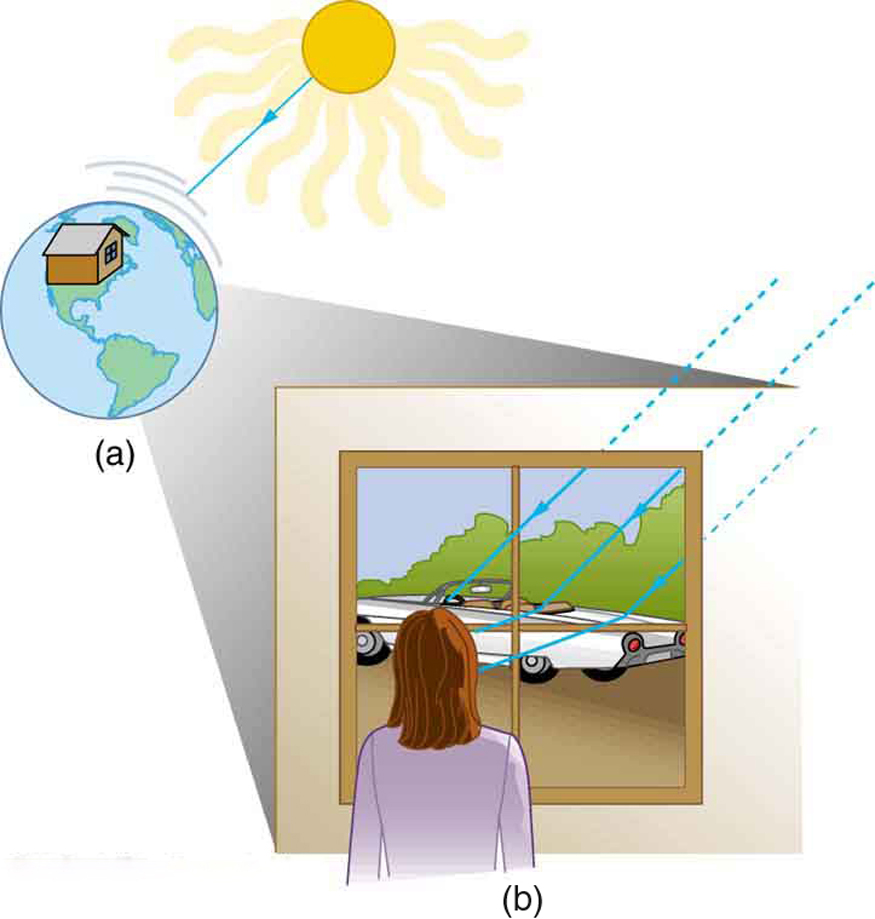
\includegraphics[scale=0.5]{source}
	\end{center}
	To understand about the direction of propagation of a wave, look at light entering a room through a small opening in a wall. You will note the motion of dust particles, which essentially provide simple evidence that light travels in a straight line. An arrow headed straight line represents the direction of propagation of light and is called a ray. Light rays are drawn using straight lines and arrow heads and are used to show the path that light travels. A collection of rays is called a beam. Light rays are, thus, narrow beam of light that travel in a straight line. You can use the idea of a light ray to indicate the direction that light travels. A ray diagram is a drawing that shows the path of light rays. Simplifying light waves as rays that travel along a straight line makes our understanding of the wave nature of light much simpler. We can use techniques such as ray-tracing to understand and predict the motion of light.   
	\subsection*{Reflection of Light}
	Whenever we look into a mirror or a newly varnished furniture, we are seeing a reflection. Even when you are reading this, too, you are seeing light reflected from it. The most important thing to remember is that you can only see an object when light from the object enters our eyes. The object must be a source of light (for example, a light bulb) or else it must reflect light from a source
	(for example, the moon), and the reflected light enters our eyes.
	\begin{center}
		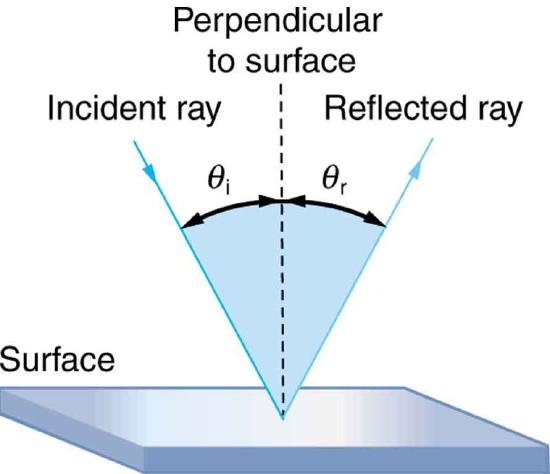
\includegraphics[scale=0.3]{reflection}
	\end{center}
	When light is facing a boundary it can not pass through, it seems as though it comes bounces back out of that boundary - this bouncing back of light rays is called reflection. There are the so called Laws of Reflection that guide us on how we expect light to travel back off of such surfaces.
	\begin{enumerate}
		\item The incident ray, the reflected ray and the normal to the plane lie on the plane.
		\item The angle of incidence and the angle of reflection are equal(measured with respect to the normal).
		\item The incident ray and the reflected ray are on the opposite sides of the normal.
	\end{enumerate}
	On the basis of the boundary that causes reflection, we can categorize reflections into two - specular and diffuse.
	\begin{center}
		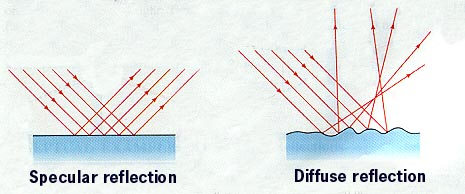
\includegraphics[scale=0.6]{reflection_types}
	\end{center}
	The reflection of light from a smooth shiny surface is
	referred to as specular reflection. Notice that all the reflected light moves in the same direction. In contrast, if a surface is rough, the reflected light is sent out in a variety of directions, giving rise to diffuse reflection. For example, when the surface of a road is wet, the water creates a smooth surface, and headlights reflecting from the road undergo specular reflection.
	\subsection*{Refraction of Light}
	The bending of a light ray when it passes through variations in matter is called refraction. Refraction is responsible for a large amount of optical phenomena, from the action of lenses to signal transmission through optical fibers. To learn why, we need to understand more about light and its motion. We might recall that light travels at a speed $c$ in vacuum, which not only is the speed of light, but is also the maximum speed in the universe while simultaneously being the one of the most important constants of nature. The speed of light does not depend on the source or the observer. However, it speed differs in the materials it penetrates through(all of which are less than its speed in vacuum.) \\ \\
	Many people through the past centuries and millennia thought light was instant - meaning that it was not bound by a finite speed, but some others performed experiments to estimate the speed of light. One such person was Ole Roemer, Roemer had noted that the average orbital period of one of Jupiter’s moons, Io, as measured from Earth, varied depending on whether Earth was moving toward or away from Jupiter. He correctly concluded that the apparent change in period was due to the change in distance between Earth and Jupiter and the time it took light to travel this distance. From his 1676 data, a value of the speed of light was calculated to be  $2.26×10^8m/s$(only 25\% different from today’s accepted value).
	\begin{center}
		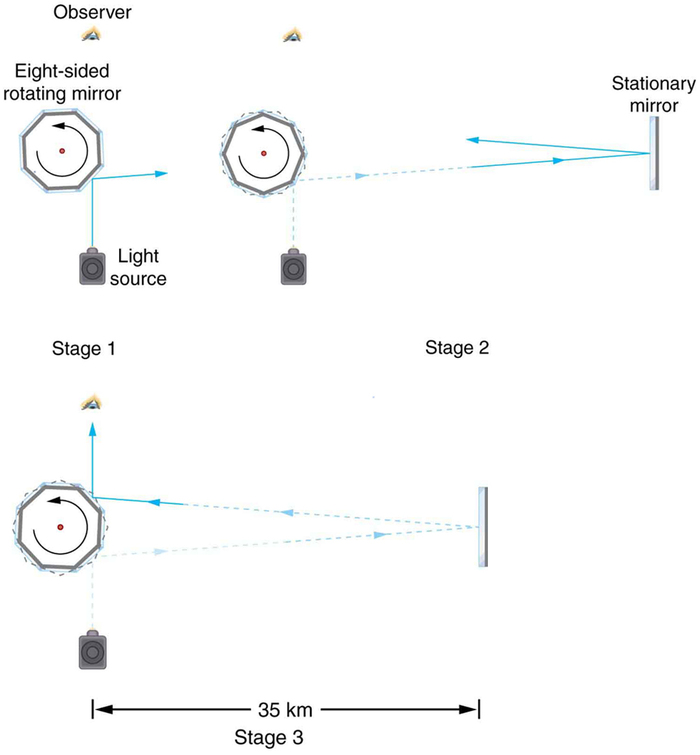
\includegraphics[scale=0.4]{michelson}
	\end{center}
	Others, such as Albert Michelson(who disproved that light needed a medium to travel through), performed an experiment by arranging an array of mirrors so that light reflected from a rotating set of mirrors was reflected from a stationary mirror 35 km away and returned to the rotating mirrors. The time for the light to travel can be determined by how fast the mirrors must rotate for the light to be returned to the observer’s eye. His results had a staggeringly small error margin of only 0.04\% to today's accepted value, which is $299,792,458m/s\approxeq3.00\times10^8m/s$. \\ \\
	When light passes through media, it speed decreases because it interacts with the matter in the media which slows it down. The amount by which light slows down in a medium compared to vacuum is defined to be the refractive index of that medium, n.
	$$n=\dfrac{c}{v}$$
	$$\text{Since }c\ge v, n\ge1$$ 
	\subsubsection*{Snell's Law}
	The Law of Refraction, also called Snell's Law tells us that The amount that a light ray changes its direction depends both on the incident angle and the amount that the speed changes. For a ray at a given incident angle, a large change in speed causes a large change in direction, and thus a large change in angle. We can state this in equation form as
	$$n_{1} \sin \theta_{i} = n_{2} \sin \theta_{r}$$
	Here, $n_1$ and  $n_2$ are the indices of refraction for medium 1 and 2, where as the angles $\theta_i$ and $\theta_i$ are the angles of incidence and refraction respectively. As with reflection, the incoming ray is called the incident ray and the outgoing ray the refracted ray, and the associated angles the incident angle and the refracted angle. \\ \\
	When light moves from a material in which its speed is
	higher to a material in which its speed is lower, such as from air to glass, the ray is bent toward the normal. If the ray moves from a material in which its speed is lower to one in which its speed is higher, the ray is bent away from the normal. If the incident ray of light is parallel to the normal, then no refraction (bending) occurs in either case. \\ \\
	We can also write Snell's law using the velocities of light in the media instead of the refractive indices.
	$$n_{1} \sin \theta_{i} = n_{2} \sin \theta_{r}$$
	$$\dfrac{c}{v_{1}} \sin \theta_{i} = \dfrac{c}{v_2}\sin \theta_{r}$$
	$$\dfrac{\sin\theta_{i}}{v_1}=\dfrac{\sin\theta_{r}}{v_2}$$
	\subsection*{Total Internal Reflection}
	Consider what is happening in the figure below.
	\begin{center}
		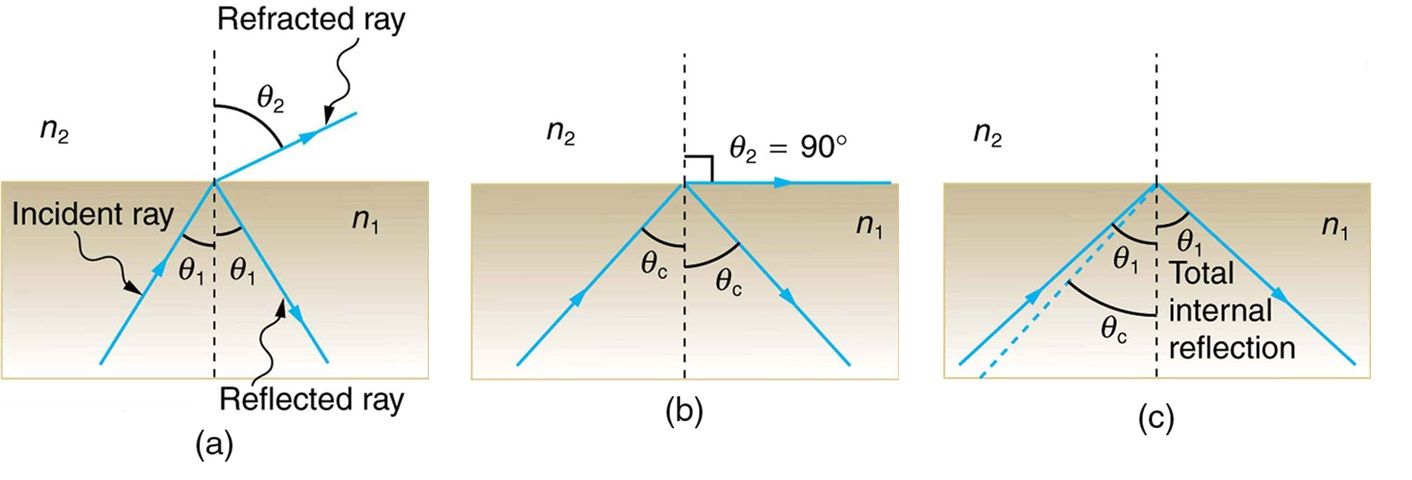
\includegraphics[scale=0.5]{tir}
	\end{center}
	Part of the light crosses the boundary and is refracted; the rest is reflected. If, as shown in the figure, the index of refraction for the second medium is less than for the first, the ray bends away from the perpendicular. There is an incident angle that causes the refraction angle to be $90^0$, that incident angle is called the critical angle. We know from Snell's law that
	$$n_{1} \sin \theta_{i} = n_{2} \sin \theta_{r}$$
	But, when we modify the above equation considering our incident is the critical angle, we get
	$$n_{1} \sin \theta_{c} = n_{2} \sin 90^0$$
	$$\sin\theta_{c}=\dfrac{n_2}{n_1}$$
	For the above to hold true, $n_2\le n_1$ because it is a sine function. Thus, for total internal reflection to occur, we have to satisfy two important preconditions
	\begin{itemize}
		\item The second medium should have a lesser refractive index than the first one
		\item The light must be incident at an angle greater than the critical angle.
	\end{itemize}
	When light undergoes total internal reflection, it actually follows through obeying the law of reflection.
	\subsubsection*{Fiber Optics}
	Fiber optics employs the transmission of light down fibers of plastic or glass. Because the fibers are thin, light entering one is likely to strike the inside surface at an angle greater than the critical angle and, thus, be totally reflected as shown in the figure below. 
	\begin{center}
		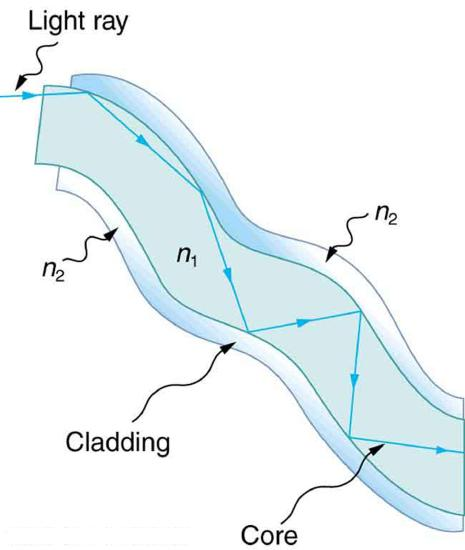
\includegraphics[scale=0.3]{fiber}
	\end{center}
	The index of refraction outside the fiber must be smaller than inside, a condition that is easily satisfied by coating the outside of the fiber with a material having an appropriate refractive index. In fact, most fibers have a varying refractive index to allow more light to be guided along the fiber through total internal refraction. Rays are reflected around corners as shown, making the fibers into tiny light pipes. \\ \\
	Fiber optics has revolutionized surgical techniques and observations within the body. The flexibility of the fiber optic bundle allows it to navigate around difficult and small regions in the body, such as the intestines, the heart, blood vessels, and joints. It also plays a major role in technology - most telephone conversations and Internet communications are now carried by laser signals along optical fibers. Extensive optical fiber cables have been placed on the ocean floor and underground to enable optical communications. Optical fiber communication systems offer several advantages over electrical (copper) based systems, especially for long distances.
	\subsection*{Dispersion}
	When our eye receives pure-wavelength light, we tend to see only one of the six colors, depending on wavelength. The thousands of other hues we can sense in other situations are our eye’s response to various mixtures of wavelengths. White light, in particular, is a fairly uniform mixture of all visible wavelengths. Sunlight, considered to be white, actually appears to be a bit yellow because of its mixture of wavelengths, but it does contain all visible wavelengths.
	\begin{center}
		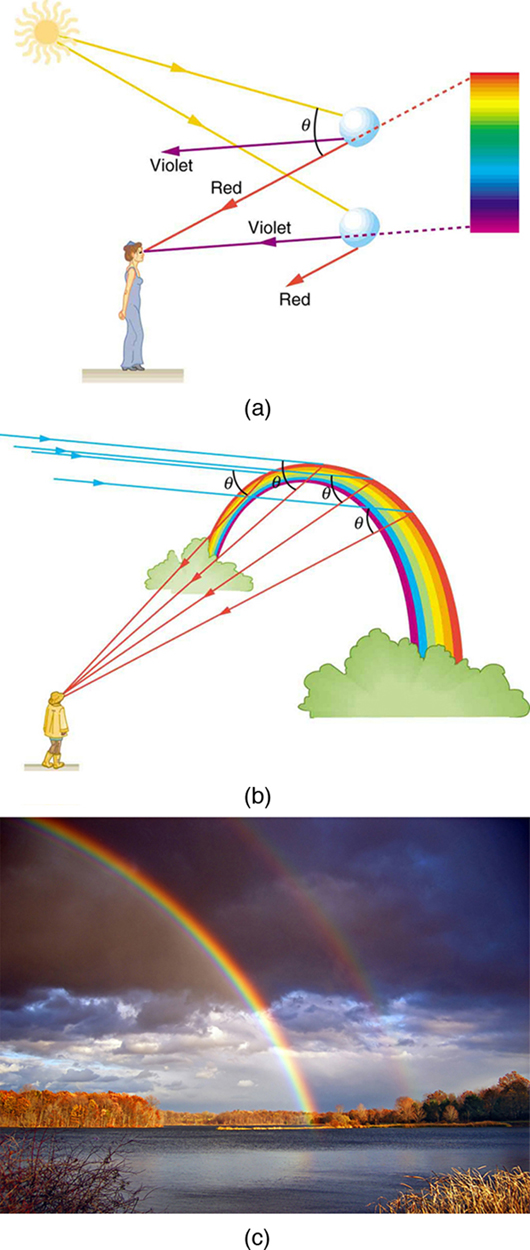
\includegraphics[scale=0.5]{Dispersion}
	\end{center}
	Dispersion is defined as the spreading of white light into its full spectrum of wavelengths. More technically, dispersion occurs whenever there is a process that changes the direction of light in a manner that depends on wavelength. Dispersion, as a general phenomenon, can occur for any type of wave and always involves wavelength-dependent processes. This happens because, for a given medium the refractive index depends on the wavelength of the light being refracted. The lower its wavelength, the more bent the light gets. \\ \\
	When rainbows are formed, for example, light enters a drop of water and is reflected from the back of the drop. The light is refracted both as it enters and as it leaves the drop. 
	\begin{center}
		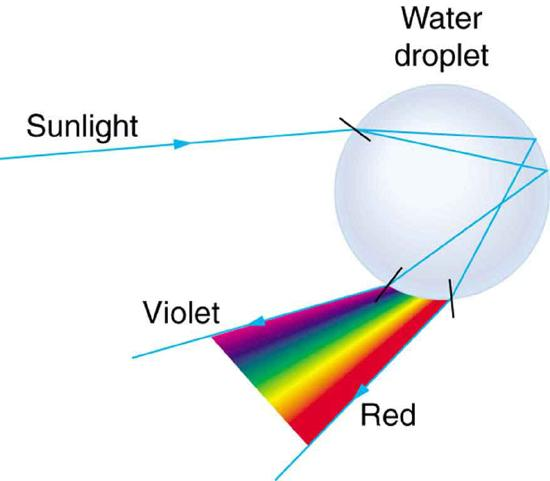
\includegraphics[scale=0.3]{droplet}
	\end{center}
	Since the index of refraction of water varies with wavelength, the light is dispersed, and a rainbow is observed. The effect is most spectacular when the background is dark, as in stormy weather, but can also be observed in waterfalls and lawn sprinklers. The arc of a rainbow comes from the need to be looking at a specific angle relative to the direction of the sun.
	\subsection*{Image formation by Lenses}
	The word lens derives from the Latin word for a lentil bean, the shape of which is similar to the convex lens. Lenses are found in a almost all optical instruments, ranging from a simple magnifying glass to the eye to a camera’s zoom lens.
	\begin{center}
		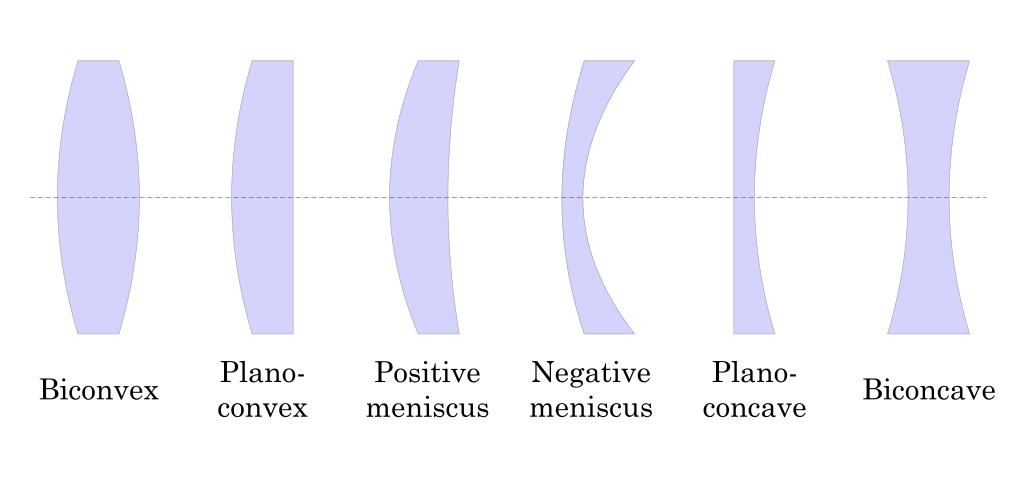
\includegraphics[scale=0.3]{lenses}
	\end{center}
	Lenses are classified by the curvature of the two optical surfaces. A lens is biconvex if both surfaces are convex. A lens with two concave surfaces is biconcave. If one of the surfaces is flat, the lens is plano-convex or plano-concave depending on the curvature of the other surface. A lens with one convex and one concave side is convex-concave or meniscus. It is this type of lens that is most commonly used in corrective lenses. 
	\subsubsection*{Converging Lenses}
	\begin{center}
		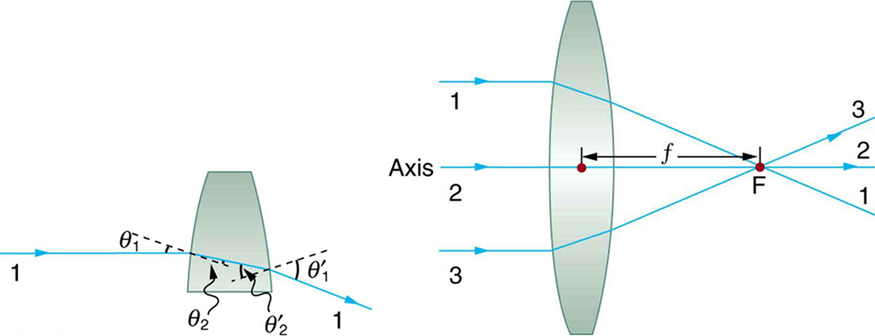
\includegraphics[scale=0.5]{convex_lens}
	\end{center}
	A convex lens is shaped so that all light rays that enter it parallel to its axis cross one another at a single point on the opposite side of the lens. (\textit{The axis is defined to be a line normal to the lens at its center}.) Such a lens is called a converging lens for the converging effect it has on light rays. The point at which the rays cross is defined to be the \textbf{focal point} F of the lens. The distance from the center of the lens to its focal point is defined to be the focal length $f$ of the lens. \\ \\
	The greater effect a lens has on light rays, the more powerful it is said to be. For example, a powerful converging lens will focus(converge) parallel light rays closer to itself and will have a smaller focal length than a weaker lens. The power of a lens is defined to be the reciprocal of its focal length.
	$$P=\dfrac{1}{f}$$
	The Power has SI units of Diopters such that $1D = \dfrac{1}{m}$ 
	\subsubsection*{Diverging Lenses}
	\begin{center}
		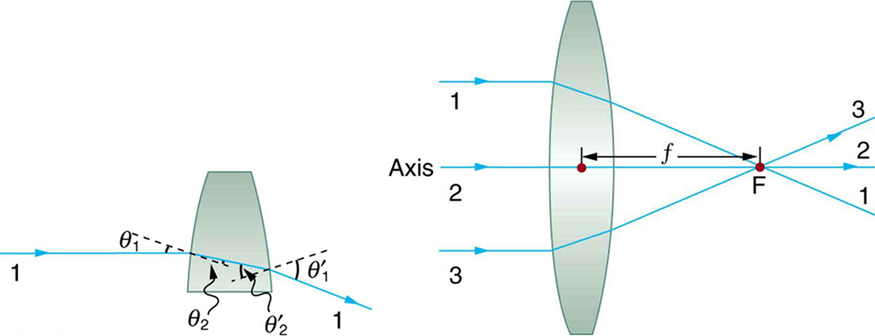
\includegraphics[scale=0.5]{convex_lens}
	\end{center}
	A concave lens is shaped so that all light rays that enter it parallel to its axis cross one another acts as if they emerge from a single point(the focal point) on the same side of the lens. One major difference here is that the focal length is defined to be negative which also makes the power negative.
	\subsection*{Thin lenses and Ray tracing}
	Whenever we are discussing the refractions due to lenses, we assume our lenses are thin. A thin lens is a lens with a thickness that is negligible compared to the radii of curvature of the lens surfaces. Thin lens approximation ignores optical effects due to the thickness of lenses and simplifies ray tracing calculations. \\ \\
	Ray tracing is the technique of determining or following (tracing) the paths that light rays take. For rays passing through matter, the law of refraction is used to trace the paths. For a thin lens, we follow simple rules to trace the image created by the lens.
	\begin{enumerate}
		\item A ray entering a converging lens parallel to its axis passes through the focal point F of the lens on the other side. 
		\item A ray entering a diverging lens parallel to its axis seems to come from the focal point F. 
		\item A ray passing through the center of either a converging or a diverging lens does not change direction. 
		\item A ray entering a converging lens through its focal point exits parallel to its axis. 
		\item A ray that enters a diverging lens by heading toward the focal point on the opposite side exits parallel to the axis. 
	\end{enumerate}
	$$\textit{If you would like to report errors that needs to be fixed, email aaron@stjohn.edu.et}$$
\end{document}	 